\section{Actividad 8}

\subsection*{En un determinado circuito se tienen tres amplificadores conectados en cascada, tal
como se puede observar en la Fig. }

    \begin{figure}[H]
        \centering
        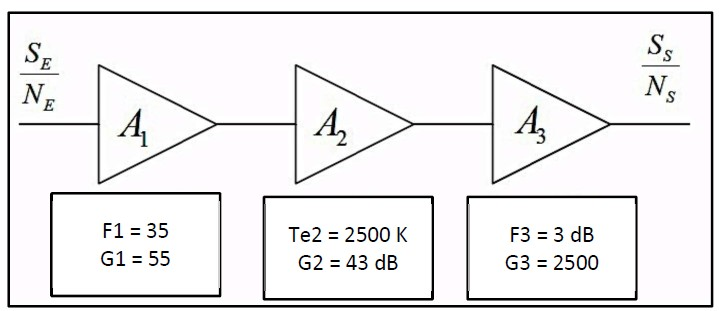
\includegraphics[width=0.8\linewidth]{imagenes/Actividad_8/actividad_8.jpg}
        \caption{Circuito en cascada.}
        \label{fig:diagrama_8}
    \end{figure}

\subsection*{Calcular:}

\subsection*{a) La figura de ruido total, suponiendo la temperatura ambiente T = 290 K.}

\subsection*{b) La temperatura equivalente de ruido total.}

\subsection*{c) Intercambiar los amplificadores A1 y A3. Calcular nuevamente la figura de ruido total, y explicar que sucede.}

\subsection*{d) Suponer que ingresa a la cascada de amplificadores una señal con una potencia de 20x10-9 W. Calcular la relación señal ruido 
tanto en la entrada, como en la salida de dicha cascada, considerando $\Delta f = 150 kHz$.}